\chapter{آزمایش‌ها و نتایج}
\clearpage

در این فصل ابتدا به معرفی مجموعه داده‌های استفاده شده در انجام آزمایش‌ها می‌پردازیم. سپس به بررسی آزمایش‌های انجام شده و نتایج به‌دست‌آمده از ارزیابی مدل پیشنهادی می‌پردازیم و نتایج حاصل را مورد بررسی قرار می‌دهیم.

به‌طور کلی، آزمایش‌های انجام شده در این پژوهش را می‌توان به دو دسته تقسیم کرد:
\begin{enumerate}
    \item پیش‌آموزش خودنظارتی بر روی مجموعه داده‌ی کوچک و تنظیم دقیق بر روی همان مجموعه.
    \item پیش‌آموزش خودنظارتی بر روی مجموعه داده‌ی بزرگ و تنظیم دقیق بر روی مجموعه داده‌ی کوچک.
\end{enumerate}

\section{مجموعه داده}

برای ارزیابی عملکرد روش پیشنهادی در این پژوهش، از دو مجموعه داده \lr{HAPT\LTRfootnote{Smartphone-Based Recognition of Human Activities and Postural Transitions}}\cite{reyes2015smartphone}
(مجموعه داده کوچک) و
\lr{MobiAct}\cite{vavoulas2016mobiact}
(مجموعه داده بزرگ)
استفاده کردیم. در ادامه، جزئیات هر یک از این مجموعه داده‌ها به تفصیل تشریح می‌شود.

\subsection{مجموعه داده \lr{HAPT}}

مجموعه داده \lr{HAPT}
یکی از مجموعه داده‌های شناخته‌شده و پرکاربرد در حوزه شناسایی فعالیت انسان است که در دسترس عموم قرار دارد. این مجموعه داده نسخه توسعه‌یافته و کامل‌تری از مجموعه داده
\lr{UCI-HAR}\cite{anguita2013public}
است و علاوه بر فعالیت‌های پایه، شامل گذارهای وضعیتی\LTRfootnote{Postural Transitions} نیز می‌شود.

هدف اصلی از ایجاد این مجموعه داده، فراهم کردن داده‌های خام و پردازش‌شده از حسگرهای اینرسی تعبیه‌شده در گوشی‌های هوشمند برای ساخت و ارزیابی مدل‌های شناسایی فعالیت است. تمرکز ویژه این مجموعه داده بر تمایز قائل شدن بین فعالیت‌های ایستا و پویا و همچنین شناسایی حرکات کوتاه و انتقالی بین حالت‌های ایستا است.

\begin{figure}[htb!]
\centering
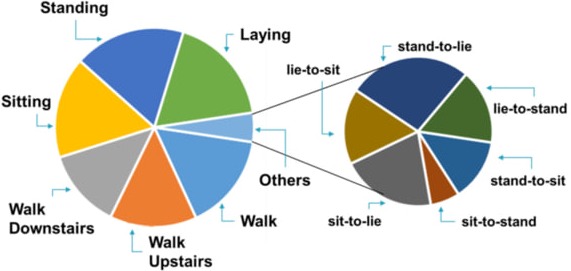
\includegraphics[width=0.75\textwidth]{Images/Chapter4/hapt-classes.png}
\caption{دسته‌های مختلف مجموعه داده \lr{HAPT}}
\label{fig:hapt-classes}
\end{figure}

داده‌های این مجموعه از ۳۰ داوطلب در بازه سنی ۱۹ تا ۴۸ سال جمع‌آوری شده است. هر شرکت‌کننده یک گوشی هوشمند \lr{Samsung Galaxy S II} را بر روی کمر خود بسته بود و رویه مشخصی از فعالیت‌ها را انجام می‌داد. تمام آزمایش‌ها به صورت ویدیویی ضبط شدند تا برچسب‌گذاری داده‌ها با دقت بالایی به صورت دستی انجام شود.

داده‌ها از دو حسگر اصلی گوشی هوشمند استخراج شده‌اند: حسگر شتاب‌سنج که سیگنال شتاب خطی سه‌محوره و حسگر ژیروسکوپ که سیگنال سرعت زاویه‌ای سه‌محوره را ثبت می‌کند. نرخ نمونه‌برداری برای هر دو حسگر ۵۰ هرتز بوده است.

همانطور که در شکل \ref{fig:hapt-classes}
می‌توان دید، این مجموعه داده شامل ۱۲ کلاس فعالیت مجزا است که به دو دسته اصلی تقسیم می‌شوند:
\begin{itemize}
    \item فعالیت‌های پایه که خود شامل سه فعالیت ایستای ایستادن، نشستن و دراز کشیدن و سه فعالیت پویای راه رفتن، بالا رفتن از پله و پایین آمدن از پله می‌باشد.
    \item گذارهای وضعیتی که شامل حرکات انتقالی بین فعالیت‌های ایستا می‌باشد و دارای فعالیت‌های ایستادن به نشستن، نشستن به ایستادن، نشستن به دراز کشیدن، دراز کشیدن به نشستن، ایستادن به دراز کشیدن و دراز کشیدن به ایستادن می‌باشد.
\end{itemize}

مجموعه داده \lr{HAPT} هم به صورت داده‌های خام حسگر و هم به صورت ویژگی‌های استخراج‌شده ارائه می‌گردد. داده‌های خام شامل سیگنال‌های سه‌محوره شتاب‌سنج و ژیروسکوپ به صورت سری زمانی است که نتیجتا شامل ۶ ویژگی می‌باشد. ویژگی‌های استخراج شده نیز بدین صورت می‌باشند که ابتدا سیگنال‌های خام با استفاده از یک پنجره لغزان به طول ۱۲۸ (۵۶.۲ ثانیه) و ۵۰ درصد همپوشانی قطعه‌بندی شده‌اند. از هر قطعه، یک بردار ویژگی ۵۶۱ بعدی استخراج شده است. این ویژگی‌ها شامل محاسبات آماری در حوزه زمان و فرکانس مانند میانگین، انحراف معیار، تبدیل فوریه سریع و غیره هستند. در این پژوهش از سیگنال‌های خام حسگرها برای آموزش مدل استفاده کردیم.

در این مجموعه داده دسته‌ی اول راه رفتن، دسته‌ی دوم بالا رفتن از پله، دسته‌ی سوم پایین آمدن از پله، دسته‌ی چهارم نشستن، دسته‌ی پنجم ایستادن، دسته‌ی ششم خوابیدن، دسته‌ی هفتم ایستادن به نشستن، دسته‌ی هشتم نشستن به ایستادن، دسته‌ی نهم نشستن به خوابیدن، دسته‌ی دهم خوابیدن به نشستن، دسته‌ی یازدهم ایستادن به خوابیدن و دسته‌ی دوازدهم خوابیدن به ایستادن می‌باشند. 

\subsection{مجموعه داده \lr{MobiAct}}

مجموعه داده \lr{MobiAct}
یک مجموعه داده عمومی برای شناسایی فعالیت انسان  است که با استفاده از حسگرهای گوشی هوشمند ایجاد شده و به طور خاص بر تشخیص فعالیت‌های روزمره و انواع سقوط\LTRfootnote{Falls}
تمرکز دارد. این مجموعه داده شامل داده‌های ثبت‌شده از سه حسگر اصلی یک گوشی هوشمند \lr{Samsung Galaxy S III}
یعنی شتاب‌سنج، ژیروسکوپ و حسگر جهت‌یاب\LTRfootnote{Orientation Sensor} می‌باشد.

داده‌ها از ۵۷ داوطلب (۴۲ مرد و ۱۵ زن) با میانگین سنی ۲۶ سال جمع‌آوری شده است. از این تعداد، ۵۰ شرکت‌کننده تمام سناریوهای مربوط به فعالیت‌های روزمره و ۵۴ شرکت‌کننده تمام سناریوهای سقوط را با موفقیت به پایان رساندند. برای شبیه‌سازی هرچه بهتر شرایط واقعی، از هر شرکت‌کننده خواسته شد تا گوشی هوشمند را به صورت آزاد و با جهت‌گیری دلخواه در جیب شلوار خود قرار دهد.

فعالیت‌های ثبت‌شده در این مجموعه داده به دو گروه اصلی تقسیم می‌شوند:
\begin{itemize}
    \item\textbf{نه نوع فعالیت روزمره:}  این فعالیت‌ها شامل ایستادن، راه رفتن، دویدن، پریدن، بالا رفتن از پله، پایین آمدن از پله، نشستن روی صندلی، وارد شدن به ماشین و خارج شدن از ماشین است.
    \item\textbf{چهار نوع سقوط شبیه‌سازی‌شده:}  این سقوط‌ها شامل سقوط به جلو، سقوط به جلو روی زانو، سقوط به پهلو و سقوط به عقب در حین تلاش برای نشستن روی صندلی می‌باشند.
\end{itemize}

\section{جزئیات پیاده‌سازی}

در این بخش به بررسی جزئیات مختلف پیاده‌سازی روش پیشنهادی (شامل پیش‌پردازش داده‌ها، آموزش مدل و معیارهای ارزیابی) می‌پردازیم.

\subsection{پیش‌پردازش داده‌ها}

پیش‌پردازش داده‌ها یک مرحله مهم در آموزش مدل‌های شناسایی فعالیت انسان است و عملکرد چشم‌گیری در بهبود نتایج به همراه دارد. برای این امر، ابتدا بایستی که داده‌ها را نرمال‌سازی کنیم. برای نرمال‌سازی داده‌ها از روش استانداردسازی که به آن نرمال‌سازی \lr{Z-score} نیز می‌گویند استفاده می‌کنیم. فرمول آن به فرم زیر است:
\begin{equation}
    z=\frac{x-\mu}{\sigma}
\end{equation}
در این رابطه $x$ بیانگر مقدار هر داده، $\mu$ بیانگر میانگین توزیع داده‌ها و $\sigma$ انحراف معیار توزیع داده‌ها می‌باشند. با استفاده از استانداردسازی، میانگین توزیع داده‌ها برابر با صفر و انحراف معیار آن‌ها برابر با یک می‌شود.

نکته‌ی مهم در رابطه با نرمال‌سازی داده‌ها این است که اگر ابتدا داده‌ی خام سیگنال‌ها را استانداردسازی کنیم و سپس تبدیل موجک را اعمال کنیم، تبدیل موجک حاصل همانطور که در شکل \ref{fig:unnormalized-wavelet}
می‌توان دید، در جاهایی که موجک استفاده شده با داده‌ی سری زمانی ورودی همبستگی بالا داشته باشد، بازه‌ی اسکالوگرام خروجی بزرگ می‌گردد و می‌تواند تا چند برابر بیشتر از داده‌ی خام سیگنال شود. به‌همین منظور، داده‌ی خام سیگنال‌ها  استانداردسازی می‌شوند و داده‌ی اسکالوگرام‌ها به‌صورت مستقل از یکدیگر استانداردسازی می‌شوند. پس از استانداردسازی داده‌ها می‌توانیم از آن‌ها برای پیش‌آموزش و آموزش مدل استفاده کنیم.

\begin{figure}[htb!]
\centering
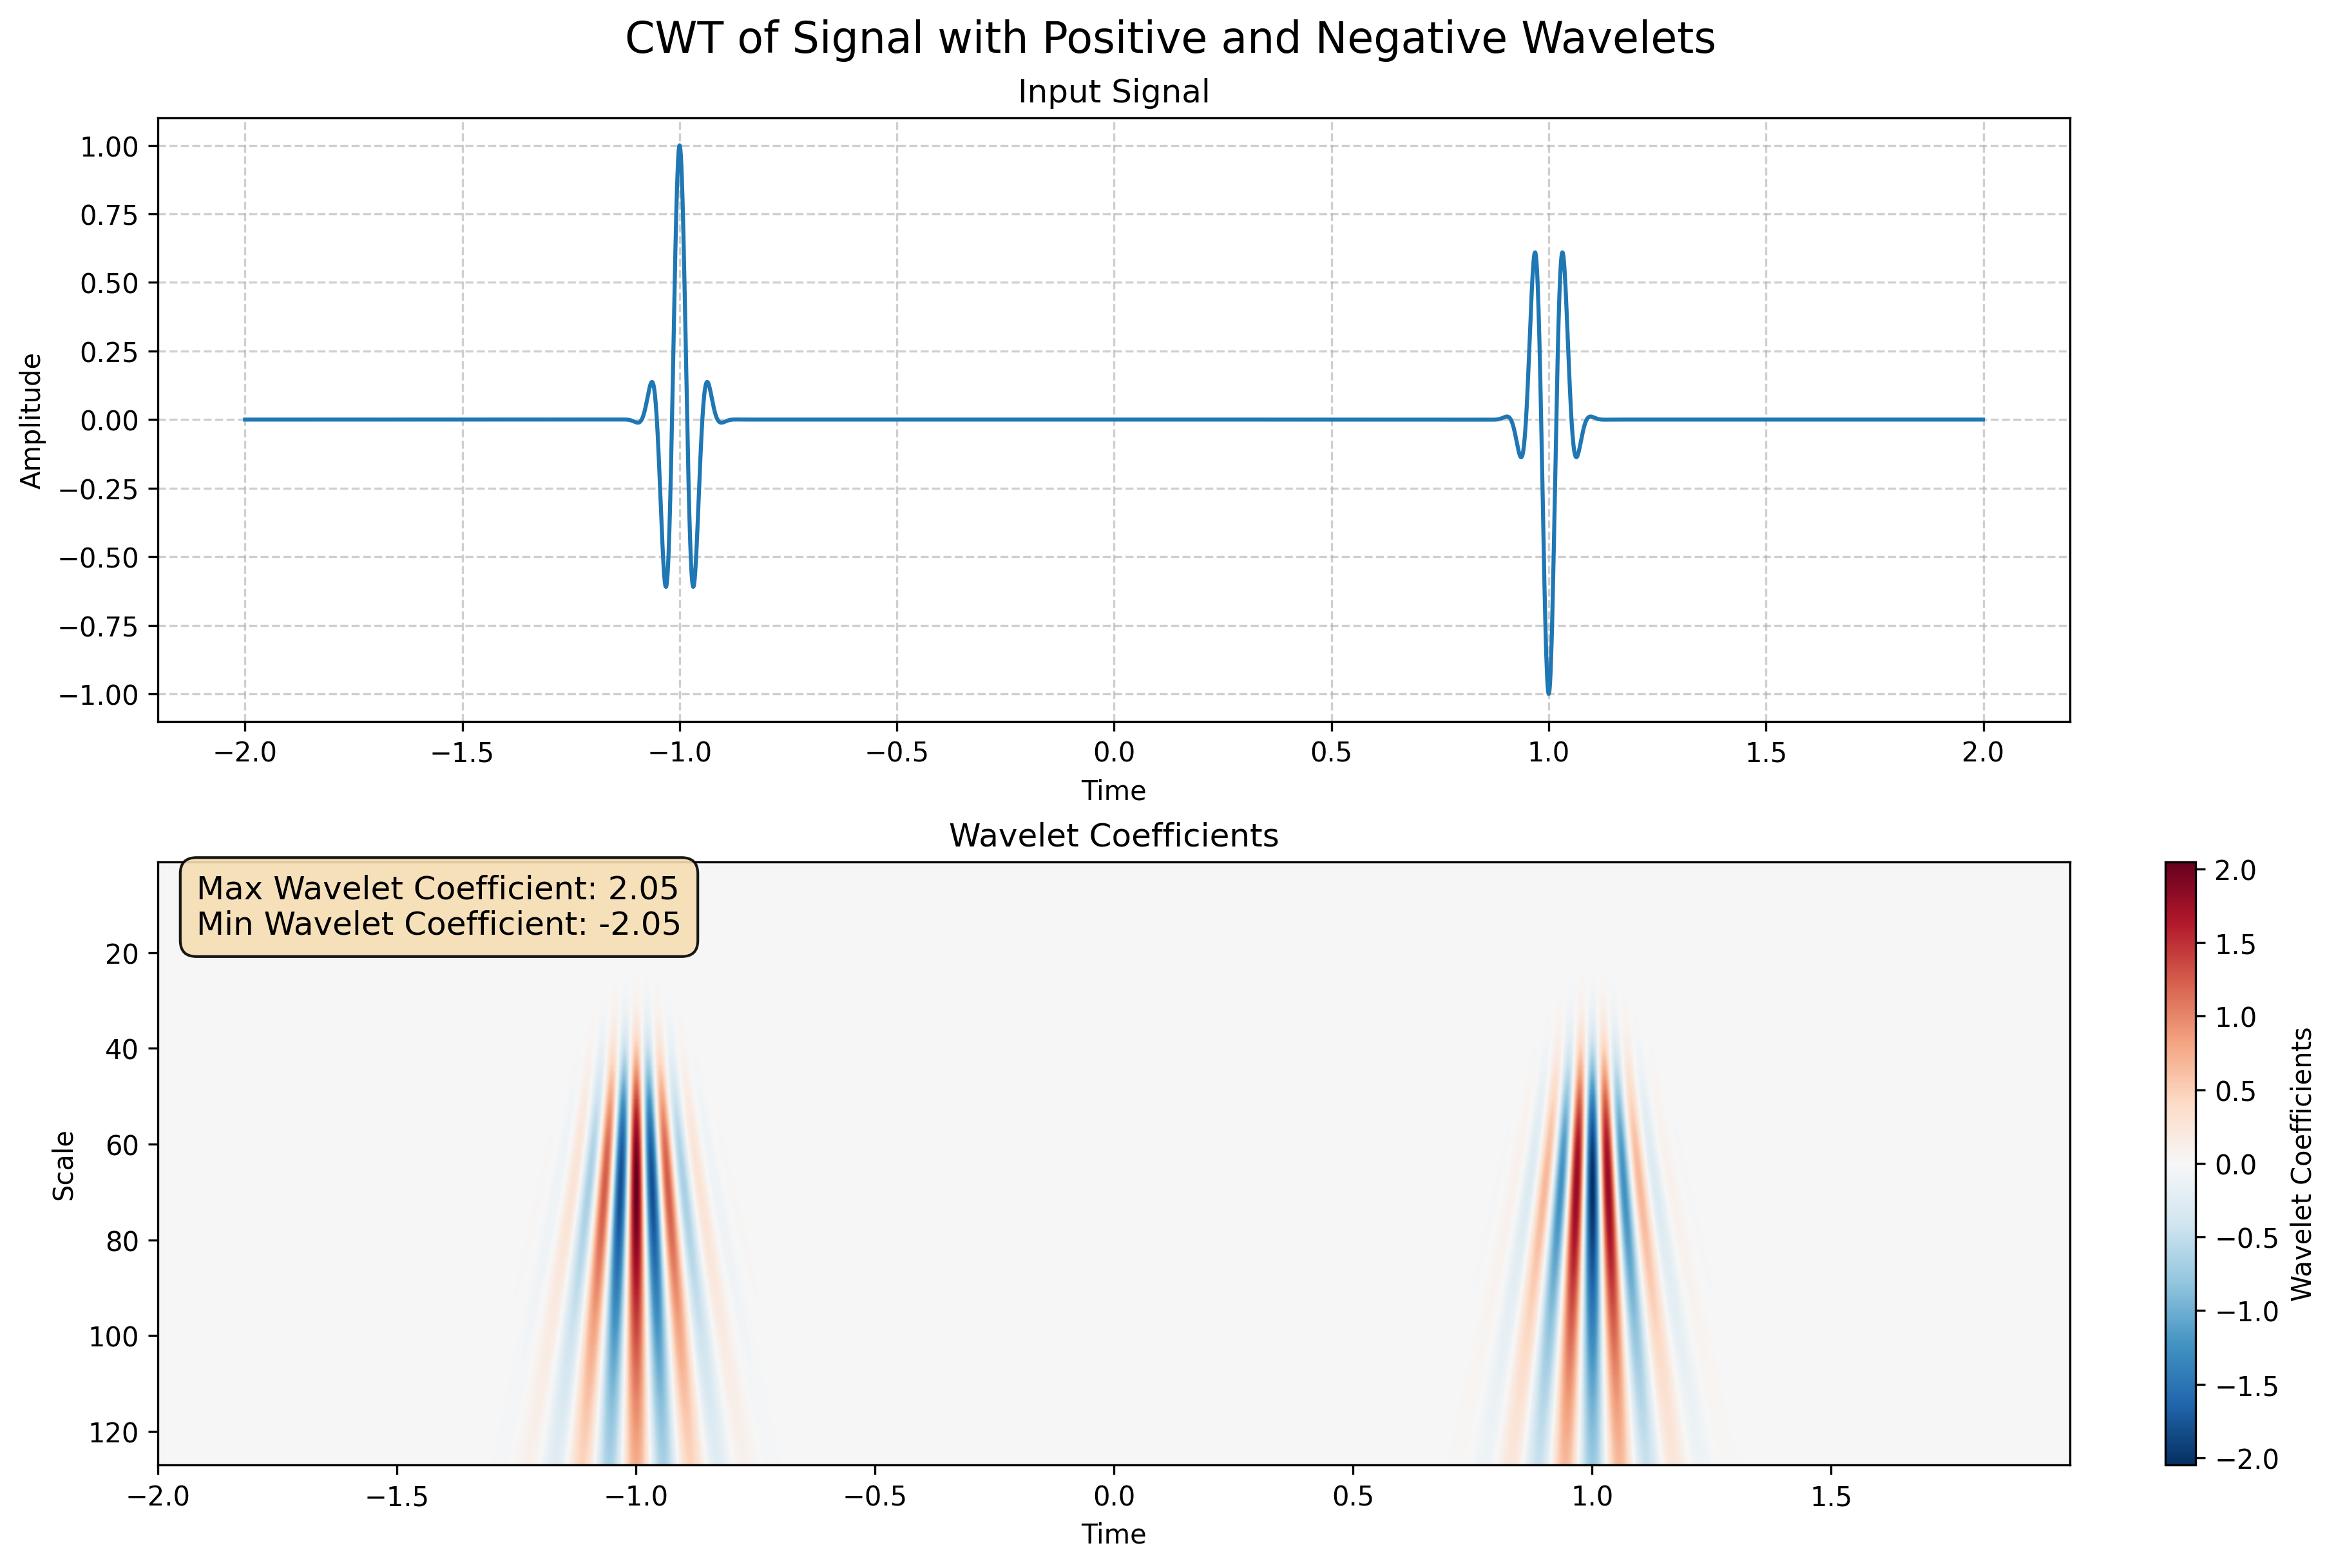
\includegraphics[width=0.75\textwidth]{Images/Chapter4/unnormalized-wavelet.png}
\caption{تاثیر تبدیل موجک بر برد اسکالوگرام خروجی}
\label{fig:unnormalized-wavelet}
\end{figure}

پس از نرمال‌سازی داده‌ها، به سراغ پر کردن مقادیر از دست رفته‌ی سیگنال‌ها با استفاده از درون‌یابی\LTRfootnote{Interpolation} می‌رویم. هر چند که هیچ یک از دو مجموعه داده‌ی استفاده شده در این پژوهش مقادیر از دست رفته ندارند، اما در هر حال می‌توان با درون‌یابی به آن‌ها رسیدگی کرد.

در قدم بعدی، بایستی نرخ نمونه‌برداری مجموعه داده‌ها را کنترل کنیم. در حالتی که هم پیش‌آموزش خودنظارتی و هم تنظیم دقیق بر روی یک مجموعه داده انجام می‌شود، نیازی به این موضوع نیست و نرخ نمونه‌برداری را همان ۵۰ هرتز
برای مجموعه داده \lr{HAPT}
نگاه می‌داریم. اما هنگامی که پیش‌آموزش بر روی مجموعه داده \lr{MobiAct}
انجام می‌شود و تنظیم دقیق بر روی \lr{HAPT}،
بایستی که هر دو مجموعه داده دارای نرخ نمونه‌برداری برابر باشند. چرا که برای مثال اگر از یک پنجره به طول ۱۰۰ استفاده کنیم، در حالتی که نرخ نمونه‌برداری ۵۰ هرتز است، به فعالیت‌های انجام شده در یک بازه‌ی ۲ ثانیه‌ای نگاه می‌کنیم. اما هنگامی که نرخ نمونه‌برداری ۲۰ هرتز باشد (نرخ نمونه‌برداری مجموعه داده \lr{MobiAct})،
به فعالیت‌های انجام شده در یک بازه‌ی ۵ ثانیه‌ای نگاه می‌کنیم. که این امر باعث افت عملکرد مدل می‌شود. به‌همین دلیل باید در حالتی که یادگیری انتقالی انجام می‌دهیم، نرخ نمونه‌برداری مجموعه داده \lr{HAPT} را نیز به ۲۰ هرتز برسانیم تا با مجموعه داده \lr{MobiAct}
هماهنگ شود.

سپس داده‌ها را به پنجره‌های لغزان به طول ۱۲۸ و دارای همپوشانی تقسیم می‌کنیم. در رابطه با مجموعه داده \lr{HAPT} به‌علت کم بودن تعداد داده‌ها میزان همپوشانی را برابر با ۹۰ درصد قرار دادیم. اما برای مجموعه داده \lr{MobiAct} میزان همپوشانی را برابر با ۵۰ درصد قرار دادیم. در تنظیم دقیق نظارت‌شده نیز برچسب هر پنجره برابر با برچسبی است که بیشترین تعداد تکرار را دارد.

\subsection{آموزش مدل}

آموزش مدل شامل دو بخش پیش‌آموزش خودنظارتی و تنظیم دقیق نظارت‌شده می‌باشد. در بخش پیش‌آموزش مدل، از تمام داده‌های موجود در مجموعه داده استفاده می‌کنیم. چرا که از برچسب داده‌ها استفاده‌ای نکرده‌ایم و صرفا هدف یادگیری توزیع داده‌ها و تولید بازنمایی مفید است. بنابراین
نشت مدل\LTRfootnote{Model leakage}
رخ نمی‌دهد.

در آموزش نظارت‌شده که از مجموعه داده \lr{HAPT} استفاده کرده‌ایم، مدل پیش‌آموزش دیده را با درصدهای مختلفی از داده‌ی آموزش و ارزیابی آموزش دادیم. این درصدها شامل ۸۰ درصد آموزش، ۶۰ درصد آموزش، ۴۰ درصد آموزش و ۲۰ درصد آموزش می‌باشند. در واقع هدف این است که قدرت تعمیم مدل و آموزش با میزان پایین داده‌ی آموزشی را ارزیابی کنیم.

روند انجام آزمایشات بدین صورت است که ابتدا کدگذارهای سیگنال و اسکالوگرام را با استفاده از روشی که در فصل قبل ارائه دادیم را پیش‌آموزش می‌دهیم و وزن‌های 
کدگذارها را ذخیره می‌کنیم. سپس در مرحله‌ی بعد، دسته‌بندها را بر روی ویژگی‌های استخراج شده از کدگذارها با استفاده از درصدهای مختلف داده آموزشی آموزش می‌دهیم. به ازا هر درصد، ۵ بار آزمایش را به‌این صورت تکرار می‌کنیم:
\begin{enumerate}
    \item مجموعه داده را به ۵ بخش مساوی تقسیم می‌کنیم.
    \item بسته به درصد داده‌ی آموزشی و ارزیابی، تعدادی از این بخش‌ها آموزشی و تعدادی از آن‌ها ارزیابی می‌باشند.
    \item ۵ بار آزمایش را تکرار می‌کنیم و هر بار داده‌های آموزشی و ارزیابی متفاوت می‌باشند.
    \item ارزیابی نهایی عملکرد مدل برابر با میانگین ۵ بار اجرا مربوطه می‌باشد.
\end{enumerate}

\subsection{معیارهای ارزیابی}

ارزیابی عملکرد مدل‌های یکی از مهم‌ترین بخش‌های یادگیری ماشین می‌باشد. در این پژوهش از دو معیار ارزیابی امتیاز \lr{F1}\LTRfootnote{F1 Score}
و امتیاز کاپا\LTRfootnote{Kappa Score}
(که به آن کاپای کوهن\LTRfootnote{Cohen's Kappa} نیز می‌گویند) استفاده کرده‌ایم. اما پیش از بررسی این دو معیار ارزیابی، بایستی که ۳ معیار ارزیابی دیگر شامل صحت\LTRfootnote{Accuracy}، دقت\LTRfootnote{Precision} و فراخوانی\LTRfootnote{Recall} را معرفی کنیم.

معیار صحت به‌عنوان یکی از معیارهای پرکاربرد برای ارزیابی یک مدل دسته‌بندی در مسائل مختلف یادگیری ماشین مورد استفاده قرار می‌گیرد. این معیار نسبت تعداد داده‌هایی را که به درستی توسط مدل دسته‌بندی شده‌اند به تعداد کل داده‌های موجود در داده‌های آزمون می‌سنجد. فرمول محاسبه صحت به فرم معادله \ref{eq:accuracy} می‌باشد:
\begin{equation}
    \mathrm{Accuracy}=\frac{TP+TN}{TP+TN+FP+FN}
    \label{eq:accuracy}
\end{equation}
در این معادله، $TP$\LTRfootnote{True Positive} به تعداد نمونه‌های مثبت واقعی که به درستی مثبت تشخیص داده‌شده‌اند، $TN$\LTRfootnote{True Negative} به تعداد نمونه‌های منفی واقعی که به درستی منفی تشخیص داده‌شده‌اند، $FP$\LTRfootnote{False Positive} به تعداد نمونه‌های منفی واقعی که به اشتباه مثبت تشخیص داده‌شده‌اند و $FN$\LTRfootnote{False Negative} به تعداد نمونه‌های مثبت واقعی که به اشتباه به‌عنوان منفی تشخیص داده‌شده‌اند اشاره دارد.

معیار دقت بیانگر نسبت نمونه‌های مثبت واقعی که به درستی تشخیص داده‌شده‌اند به تعداد نمونه‌هایی که مدل مثبت تشخیص داده‌است می‌باشد:
\begin{equation}
    \mathrm{Precision}=\frac{TP}{TP+FP}
\end{equation}
معیار فراخوانی نیز بیانگر نسبت نمونه‌های مثبت واقعی که به درستی تشخیص داده‌شده‌اند به تعداد کل نمونه‌های مثبت واقعی است:
\begin{equation}
    \mathrm{Recall}=\frac{TP}{TP+FN}
\end{equation}
حال به بررسی معیارهای ارزیابی مورد استفاده در این پژوهش می‌پردازیم. معیار امتیاز \lr{F1}
یک معیار جامع برای ارزیابی مدل‌های دسته‌بندی است که به صورت ترکیبی از دقت و فراخوانی محاسبه می‌شود. این معیار بیشتر منعکس‌کننده‌ی توازن میان دقت و فراخوانی مدل است. فرمول محاسبه امتیاز \lr{F1} به فرم معادله \ref{eq:f1-score} می‌باشد:
\begin{equation}
    \mathrm{F1 \space Score}=2\times\frac{\mathrm{Precision}\times\mathrm{Recall}}{\mathrm{Precision}+\mathrm{Recall}}
    \label{eq:f1-score}
\end{equation}
معیار ارزیابی دیگری که در این پژوهش مورد استفاده قرار گرفته است، امتیاز کاپا می‌باشد. این معیار، میزان توافق بین پیش‌بینی‌های انجام‌شده توسط مدل و برچسب‌های واقعی را با در نظر گرفتن احتمال توافق تصادفی، ارزیابی می‌کند. مزیت اصلی امتیاز کاپا این است که نشان می‌دهد عملکرد مدل تا چه حد از یک حدس کاملاً تصادفی بهتر است. این ویژگی، کاپا را به معیاری قابل اطمینان‌تر، به‌ویژه در هنگام مواجهه با مجموعه داده‌های نامتوازن تبدیل می‌کند. فرمول محاسبه امتیاز کاپا به فرم معادله \ref{eq:kappa} می‌باشد:
\begin{equation}
\mathrm{Kappa} = \frac{\mathrm{Accuracy} - \mathrm{Accuracy_r}}{1 - \mathrm{Accuracy_r}}
\label{eq:kappa}
\end{equation}
در این معادله،
\lr{Accuracy}
همان صحت مدل است و $\mathrm{Accuracy}_r$
نشان‌دهنده‌ی صحت توافق تصادفی است. این مقدار، نمایانگر صحت عملکرد یک مدل فرضی است که تعداد پیش‌بینی‌هایش برای هر دسته، دقیقا با تعداد پیش‌بینی‌های مدل اصلی ما یکسان است، اما این تخصیص برچسب‌ها را کاملا 
به صورت تصادفی انجام می‌دهد. به عبارت دیگر، ما عملکرد مدل خود را با یک پیش‌بینی‌کننده‌ی تصادفی که از توزیع داده‌ها آگاه است، مقایسه می‌کنیم تا ببینیم یادگیری مدل چقدر فراتر از شانس بوده است. برای یک مسئله‌ی دسته‌بندی چندکلاسه با $k$
دسته، فرمول کلی محاسبه‌ی $\mathrm{Accuracy}_r$
به صورت معادله \ref{eq:acc_r_multiclass} می‌باشد:
\begin{equation}
\mathrm{Accuracy_r} = \frac{1}{N^2} \sum_{i=1}^{k} (A_i \times P_i)
\label{eq:acc_r_multiclass}
\end{equation}
در این معادله $k$ تعداد دسته‌ها، $N$ تعداد کل نمونه‌ها، $A_i$ تعداد کل نمونه‌های واقعی متعلق به دسته‌ی $i$ و $P_i$
تعداد کل نمونه‌هایی است که توسط مدل به عنوان دسته‌ی $i$ پیش‌بینی شده‌اند.

مقدار امتیاز کاپا بین ۱- و ۱+ قرار دارد. مقادیر مثبت به معنای عملکرد بهتر مدل از یک دسته‌بند تصادفی، مقدار صفر به معنای عملکرد کاملا تصادفی مدل و مقادیر منفی به معنای عملکرد بدتر مدل از یک دسته‌بند تصادفی می‌باشد.

\subsection{ابرپارامترها}

جزئیات پیکربندی مدل پیشنهادی در جدول \ref{tab:model-configs}
قابل مشاهده می‌باشد. مقادیر انتخابی بر اساس روش پایه \cite{taghanaki2023self} انتخاب شده‌اند و جستجوی گسترده‌ای برای یافتن پیکربندی بهینه انجام نشده است. تعداد خوشه‌ها برای روش \lr{SwAV} نیز به‌صورت تجربی بایستی حدود ۱۰ برابر تعداد دسته‌های مجموعه داده هدف باشند\cite{caron2020unsupervised}. بنابراین تعداد خوشه‌ها را برابر با ۱۲۸ قرار دادیم.

\begin{table}[ht]
\centering
\caption{پیکربندی یادگیرنده‌ی سیگنال (سمت راست) و یادگیرنده‌ی اسکالوگرام (سمت چپ)}
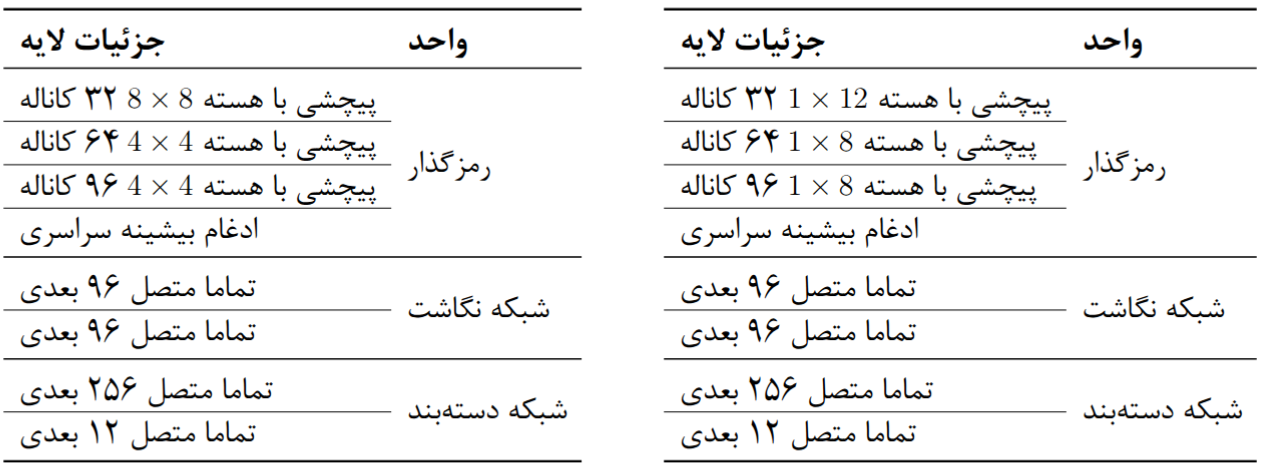
\includegraphics[width=1\textwidth]{Images/Chapter4/structure-table.png}
\label{tab:model-configs}
\end{table}

% \begin{table}[h]
% \centering
% \caption{پیکربندی یادگیرنده‌ی سیگنال (سمت راست) و یادگیرنده‌ی اسکالوگرام (سمت چپ)}
% \label{tab:model-configs}

% % ------------ جدول اول ------------
% \begin{minipage}{0.4\textwidth}
% \centering
% \renewcommand{\arraystretch}{1.2} % تنظیم فاصله عمودی بین ردیف‌ها
% \begin{tabular}{ll} % حذف خطوط عمودی
%     \toprule % خط افقی بالایی ضخیم
%     \textbf{واحد} & \textbf{جزئیات لایه} \\
%     \midrule % خط افقی میانی
%     \multirow{4}{*}{کدگذار} & پیچشی با هسته \lr{$1 \times 12$} ۳۲ کاناله \\
%     \cline{2-2} % خط افقی فقط برای ستون دوم
%     & پیچشی با هسته \lr{$1 \times 8$} ۶۴ کاناله \\
%     \cline{2-2}
%     & پیچشی با هسته \lr{$1 \times 8$} ۹۶ کاناله \\
%     \cline{2-2}
%     & ادغام بیشینه سراسری \\
%     \midrule % خط افقی میانی
%     \multirow{2}{*}{شبکه نگاشت} & تماما متصل ۹۶ بعدی \\
%     \cline{2-2}
%     & تماما متصل ۹۶ بعدی \\
%     \midrule % خط افقی میانی
%     \multirow{2}{*}{شبکه دسته‌بند} & تماما متصل ۲۵۶ بعدی \\
%     \cline{2-2}
%     & تماما متصل ۱۲ بعدی \\
%     \bottomrule % خط افقی پایینی ضخیم
% \end{tabular}
% \end{minipage}
% \hfill % ایجاد فاصله افقی بین دو جدول
% % ------------ جدول دوم ------------
% \begin{minipage}{0.4\textwidth}
% \centering
% \renewcommand{\arraystretch}{1.2} % تنظیم فاصله عمودی بین ردیف‌ها
% \begin{tabular}{ll} % حذف خطوط عمودی
%     \toprule % خط افقی بالایی ضخیم
%     \textbf{واحد} & \textbf{جزئیات لایه} \\
%     \midrule % خط افقی میانی
%     \multirow{4}{*}{کدگذار} & پیچشی با هسته \lr{$8 \times 8$} ۳۲ کاناله \\
%     \cline{2-2} % خط افقی فقط برای ستون دوم
%     & پیچشی با هسته \lr{$4 \times 4$} ۶۴ کاناله \\
%     \cline{2-2}
%     & پیچشی با هسته \lr{$4 \times 4$} ۹۶ کاناله \\
%     \cline{2-2}
%     & ادغام بیشینه سراسری \\
%     \midrule % خط افقی میانی
%     \multirow{2}{*}{شبکه نگاشت} & تماما متصل ۹۶ بعدی \\
%     \cline{2-2}
%     & تماما متصل ۹۶ بعدی \\
%     \midrule % خط افقی میانی
%     \multirow{2}{*}{شبکه دسته‌بند} & تماما متصل ۲۵۶ بعدی \\
%     \cline{2-2}
%     & تماما متصل ۱۲ بعدی \\
%     \bottomrule % خط افقی پایینی ضخیم
% \end{tabular}
% \end{minipage}
% \end{table}

نرخ یادگیری در بخش پیش‌آموزش خودنظارتی بدین صورت می‌باشد:
\begin{enumerate}
    \item مقدار اولیه‌ی نرخ یادگیری را برابر با $0.001$ قرار می‌دهیم.
    \item به‌صورت خطی طی ۱۰ دوره\LTRfootnote{Epoch} اول آن را تا $0.05$ افزایش می‌دهیم. مقادیر بزرگ‌تر موجب ناپایداری یادگیری می‌شوند.
    \item به صورت کسینوسی و تا آخرین دوره آموزش (۱۰۰ دوره) مقدار نرخ یادگیری را تا $0.0001$ کاهش می‌دهیم.
\end{enumerate}
برای تنظیم دقیق مدل، از یک نرخ یادگیری ثابت برابر با $0.001$ استفاده کردیم.
تعداد تکرار الگوریتم سینکهورن (که در بخش \ref{sec:sinkhorn} معرفی کردیم) برابر با ۳ می‌باشد.

مقدار ابرپارمتر $\epsilon$ (معادله \ref{eq:swav-optimal-transport}) را برابر با $0.01$ قرار دادیم. افزایش مقدار این پارامتر باعث می‌شود که تخصیص‌های روش سینکهورن برای تمامی داده‌ها به تمامی خوشه‌ها یکنواخت شود که در این حالت مدل بازنمایی‌های خوبی یاد نمی‌گیرد. پارامتر دما ($\tau$ در معادله \ref{eq:swav-p-calculation}) نیز می‌تواند تاثیری مشابه داشته باشد. زیاد کردن مقدار آن باعث می‌شود که توزیع تخصیص‌ها توسط مدل (نه الگوریتم سینکهورن) یکنواخت شود. اما بیش از حد کم کردن مقدار آن نیز شدیدا باعث ناپایداری آموزش خواهد شد. همانطور که در معادله \ref{eq:swav-p-calculation} دیده می‌شود،
مقدار موجود در نمای $exp$ تقسیم بر ابرپارمتر دما می‌شود. کوچک بودن بیش از حد این ابرپارامتر باعث می‌شود که مقدار این توان از لحاظ عددی بسیار بزرگ شود که به تبع آن کامپیوتر نمی‌تواند مقدار آن را محاسبه کند و فرایند آموزش دچار  خطا می‌شود. بنابراین مقدار آن را برابر با مقدار $0.05$ قرار دادیم که هم از یکنواخت شدن توزیع سینکهورن جلوگیری می‌کند و هم باعث ناپایداری آموزش نمی‌شود.

اندازه‌ی دسته برای داده‌های خام سیگنال را برابر با ۱۰۲۴ و برای اسکالوگرام نیز برابر با ۵۱۲ قرار دادیم. تعداد دوره‌ی آموزش در بخش پیش‌آموزش خودنظارتی را برای کدگذار سیگنال برابر با ۱۰۰ و برای کدگذار اسکالوگرام برابر با ۷۵ قرار دادیم. اما برای تنظیم دقیق هر دو مدل، از روش توقف زودهنگام\LTRfootnote{Early Stopping}
استفاده می‌کنیم. بدین صورت که بر روی داده‌های اعتبارسنجی، مقدار هزینه مدل را بررسی می‌کنیم و هنگامی که مدل دچار بیش‌برازش شد و هزینه‌ی اعتبارسنجی بالا رفت، آموزش را متوقف می‌کنیم و بهترین مدل را انتخاب می‌کنیم.

\section{نتایج}

در این بخش، به ارائه و تحلیل نتایج حاصل از آزمایش‌های انجام‌شده بر روی مدل پیشنهادی پرداخته می‌شود. همانطور که پیش‌تر تشریح شد، ارزیابی عملکرد مدل در دو سناریوی اصلی صورت گرفته است. ابتدا، نتایج حاصل از پیش‌آموزش خودنظارتی و تنظیم دقیق بر روی مجموعه داده واحد \lr{HAPT}
در قالب آزمایش‌های درون‌مجموعه‌ای\LTRfootnote{Intra-Dataset} بررسی می‌گردد.
سپس، کارایی روش در سناریوی یادگیری انتقالی، که در آن پیش‌آموزش بر روی مجموعه داده \lr{MobiAct}
و تنظیم دقیق بر روی مجموعه داده \lr{HAPT}
انجام شده، تحت عنوان آزمایش‌های بین‌مجموعه‌ای\LTRfootnote{Inter-Dataset} ارائه می‌گردد.
عملکرد مدل در تمامی آزمایش‌ها با استفاده از معیارهای امتیاز
\lr{F1}
و امتیاز کاپا سنجیده شده و نتایج به تفکیک مورد بحث قرار خواهند گرفت.

\subsection{نتایج آزمایش‌های درون‌مجموعه‌ای}

در این بخش، به بررسی نتایج حاصل از سناریوی اول، یعنی پیش‌آموزش خودنظارتی و تنظیم دقیق مدل بر روی مجموعه داده‌ی \lr{HAPT}
می‌پردازیم. هدف از این آزمایش، ارزیابی عملکرد مدل در مقایسه با مدل پایه و یادگیری نظارت‌شده و ایجاد یک خط معیار برای مقایسه با نتایج یادگیری انتقالی است که در بخش بعد ارائه خواهد شد.

نتایج دقیق این آزمایش‌ها در جدول
\ref{tab:intra-dataset-comparison}
ارائه شده است. این جدول، میانگین و انحراف معیار امتیاز
\lr{F1}
و امتیاز کاپا را به ازای استفاده از ۲۰، ۴۰، ۶۰ و ۸۰ درصد از داده‌های آموزشی برچسب‌دار، پس از ۵ بار تکرار آزمایش، نمایش می‌دهد.

% \begin{LTR}
% \begin{table}[ht]
% \centering
% \caption{نتایج عملکرد مدل در سناریوی درون‌مجموعه‌ای بر اساس درصدهای مختلف داده آموزشی}
% \label{tab:intra-dataset-comparison}
% \begin{tabular}{llll}
%     \toprule
%     \textbf{\lr{Labeled Data (\%)}} & \textbf{\lr{Method}} & \textbf{\lr{F1-Score}} & \textbf{\lr{Kappa Score}} \\
%     \midrule
%     \multirow{3}{*}{\lr{20\%}} 
%     & \lr{Fully Supervised} & \lr{$0.XX \pm 0.XX$} & \lr{$0.XX \pm 0.XX$} \\
%     & \lr{Baseline \cite{taghanaki2023self}} & \lr{$0.XX \pm 0.XX$} & \lr{\textbf{$0.XX \pm 0.XX$}} \\
%     & \lr{Proposed Method (Ours)} & \lr{\textbf{$0.XX \pm 0.XX$}} & \lr{$0.XX \pm 0.XX$} \\
%     \midrule
%     \multirow{3}{*}{\lr{40\%}} 
%     & \lr{Fully Supervised} & \lr{$0.XX \pm 0.XX$} & \lr{$0.XX \pm 0.XX$} \\
%     & \lr{Baseline \cite{taghanaki2023self}} & \lr{$0.XX \pm 0.XX$} & \lr{$0.XX \pm 0.XX$} \\
%     & \lr{Proposed Method (Ours)} & \lr{\textbf{$0.XX \pm 0.XX$}} & \lr{\textbf{$0.XX \pm 0.XX$}} \\
%     \midrule
%     \multirow{3}{*}{\lr{60\%}} 
%     & \lr{Fully Supervised} & \lr{$0.XX \pm 0.XX$} & \lr{$0.XX \pm 0.XX$} \\
%     & \lr{Baseline \cite{taghanaki2023self}} & \lr{$0.XX \pm 0.XX$} & \lr{$0.XX \pm 0.XX$} \\
%     & \lr{Proposed Method (Ours)} & \lr{\textbf{$0.XX \pm 0.XX$}} & \lr{\textbf{$0.XX \pm 0.XX$}} \\
%     \midrule
%     \multirow{3}{*}{\lr{80\%}} 
%     & \lr{Fully Supervised} & \lr{$0.XX \pm 0.XX$} & \lr{$0.XX \pm 0.XX$} \\
%     & \lr{Baseline \cite{taghanaki2023self}} & \lr{$0.XX \pm 0.XX$} & \lr{$0.XX \pm 0.XX$} \\
%     & \lr{Proposed Method (Ours)} & \lr{\textbf{$0.XX \pm 0.XX$}} & \lr{\textbf{$0.XX \pm 0.XX$}} \\
%     \bottomrule
% \end{tabular}
% \end{table}
% \end{LTR}

\begin{table}[ht]
\centering
\caption{نتایج عملکرد مدل در سناریوی درون‌مجموعه‌ای بر اساس درصدهای مختلف داده آموزشی}
\label{tab:intra-dataset-comparison}
\begin{tabular}{clll}
    \toprule
    \textbf{درصد داده} & \textbf{روش} & \textbf{امتیاز \lr{F1}} & \textbf{امتیاز کاپا} \\
    \midrule
    \multirow{3}{*}{\%۲۰} 
    & کاملا نظارت‌شده & $0.439 \pm 0.006$ & $0.316 \pm 0.007$ \\
    & روش پایه \cite{taghanaki2023self} & $0.645 \pm 0.005$ & $0.554 \pm 0.008$ \\
    & روش پیشنهادی & $\boldsymbol{0.658 \pm 0.005}$ & $\boldsymbol{0.571 \pm 0.007}$ \\
    \midrule
    \multirow{3}{*}{\%۴۰} 
    & کاملا نظارت‌شده & $0.619 \pm 0.008$ & $0.521 \pm 0.008$ \\
    & روش پایه \cite{taghanaki2023self} & $\boldsymbol{0.807 \pm 0.008}$ & $\boldsymbol{0.758 \pm 0.011}$ \\
    & روش پیشنهادی & $0.806 \pm 0.009$ & $0.757 \pm 0.011$ \\
    \midrule
    \multirow{3}{*}{\%۶۰} 
    & کاملا نظارت‌شده & $0.770 \pm 0.008$ & $0.710 \pm 0.010$ \\
    & روش پایه \cite{taghanaki2023self} & $0.876 \pm 0.006$ & $0.847 \pm 0.007$ \\
    & روش پیشنهادی & $\boldsymbol{0.895 \pm 0.003}$ & $\boldsymbol{0.872 \pm 0.004}$ \\
    \midrule
    \multirow{3}{*}{\%۸۰} 
    & کاملا نظارت‌شده & $0.893 \pm 0.007$ & $0.869 \pm 0.008$ \\
    & روش پایه \cite{taghanaki2023self} & $0.914 \pm 0.013$ & $0.896 \pm 0.016$ \\
    & روش پیشنهادی & $\boldsymbol{0.923 \pm 0.007}$ & $\boldsymbol{0.907 \pm 0.009}$ \\
    \bottomrule
\end{tabular}
\end{table}

\begin{figure}[ht!]
    \centering
    \begin{subfigure}[b]{0.49\textwidth}
        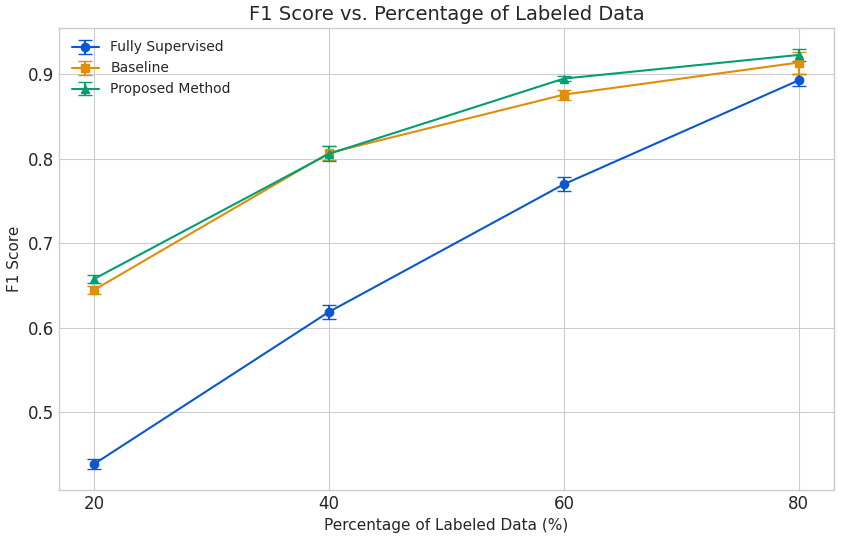
\includegraphics[width=\textwidth]{Images/Chapter4/main-results-f1.png}
    \end{subfigure}
    \hfill % ایجاد فاصله بین دو عکس
    \begin{subfigure}[b]{0.49\textwidth}
        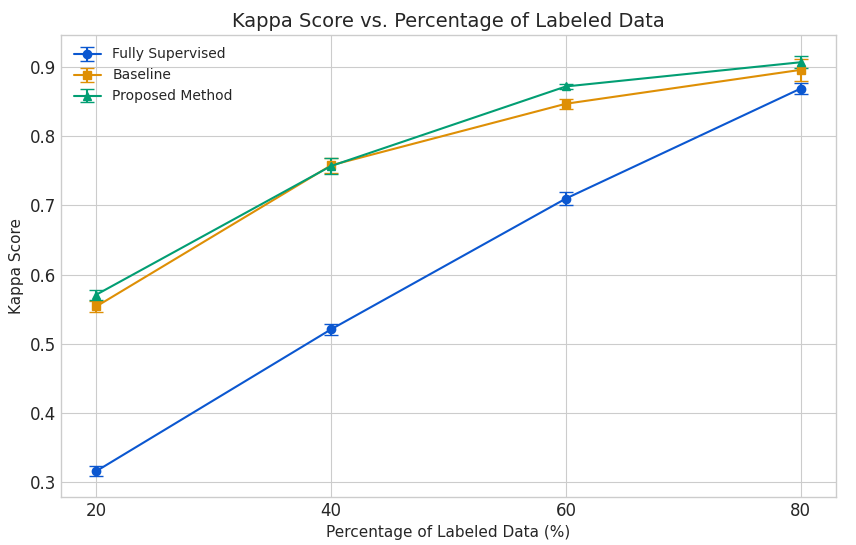
\includegraphics[width=\textwidth]{Images/Chapter4/main-results-kappa.png}
    \end{subfigure}
    \caption{مقایسه امتیاز \lr{F1} (راست) و امتیاز کاپا (چپ) برای روش‌های مختلف بر اساس درصدهای متفاوت داده‌های آموزشی.}
    \label{fig:main-results}
\end{figure}

اولین و واضح‌ترین نتیجه‌گیری که از روی جدول \ref{tab:intra-dataset-comparison} و شکل \ref{fig:main-results} می‌توان استنباط کرد، عملکرد به مراتب بهتر هر دو روش خودنظارتی (روش پایه و روش پیشنهادی) در مقایسه با روش کاملا نظارت‌شده است؛ به‌ویژه در شرایط کمبود داده‌های برچسب‌دار. برای مثال، در حالت استفاده از تنها \%۲۰ داده‌ها، روش پیشنهادی بهبودی در حدود \%۲۲ در امتیاز \lr{F1} نسبت به مدل کاملاً نظارت‌شده نشان می‌دهد.
این شکاف عمیق، ارزش مرحله پیش‌آموزش را به اثبات می‌رساند؛ جایی که مدل با استفاده از کل داده‌های برچسب‌نخورده، بازنمایی‌های غنی و مفیدی را می‌آموزد و با یک دانش اولیه قدرتمند وارد مرحله تنظیم دقیق می‌شود.

با تمرکز بر مقایسه دو روش خودنظارتی، مشاهده می‌شود که روش پیشنهادی در اکثر سناریوها (\%۲۰، \%۶۰ و \%۸۰ داده) عملکرد بهتری از خود نشان داده است.
\begin{itemize}
    \item \textbf{در شرایط داده بسیار کم (\%۲۰)}: روش پیشنهادی با اختلاف کمی، بهترین عملکرد را ثبت کرده است. این موضوع اهمیت ویژه‌ای دارد، زیرا نشان می‌دهد مدل پیشنهادی در چالش‌برانگیزترین حالت (کمبود داده) کارآمدتر است. این موضوع نشان می‌دهد که مدل پیشنهادی قابلیت تعمیم‌پذیری بیشتری می‌تواند از خود نشان بدهد.
    \item \textbf{در شرایط داده متوسط (\%۴۰):} عملکرد دو روش بسیار نزدیک و رقابتی است و روش پایه برتری جزئی و از نظر آماری نامحسوسی دارد. این نشان می‌دهد که هر دو روش در این سطح از داده به پایداری عملکردی خوبی رسیده‌اند.
    \item \textbf{در شرایط داده زیاد (\%۶۰ و \%۸۰):} با افزایش حجم داده‌های برچسب‌دار، برتری روش پیشنهادی مجدداً خود را نشان می‌دهد و به ویژه در سطح \%۶۰، شکاف قابل توجهی ایجاد می‌کند. این امر نشان‌دهنده ظرفیت بالاتر مدل پیشنهادی برای بهره‌برداری از داده‌های بیشتر و رسیدن به دقت بالاتر است.
\end{itemize}

\begin{figure}[htb!]
  \centering
  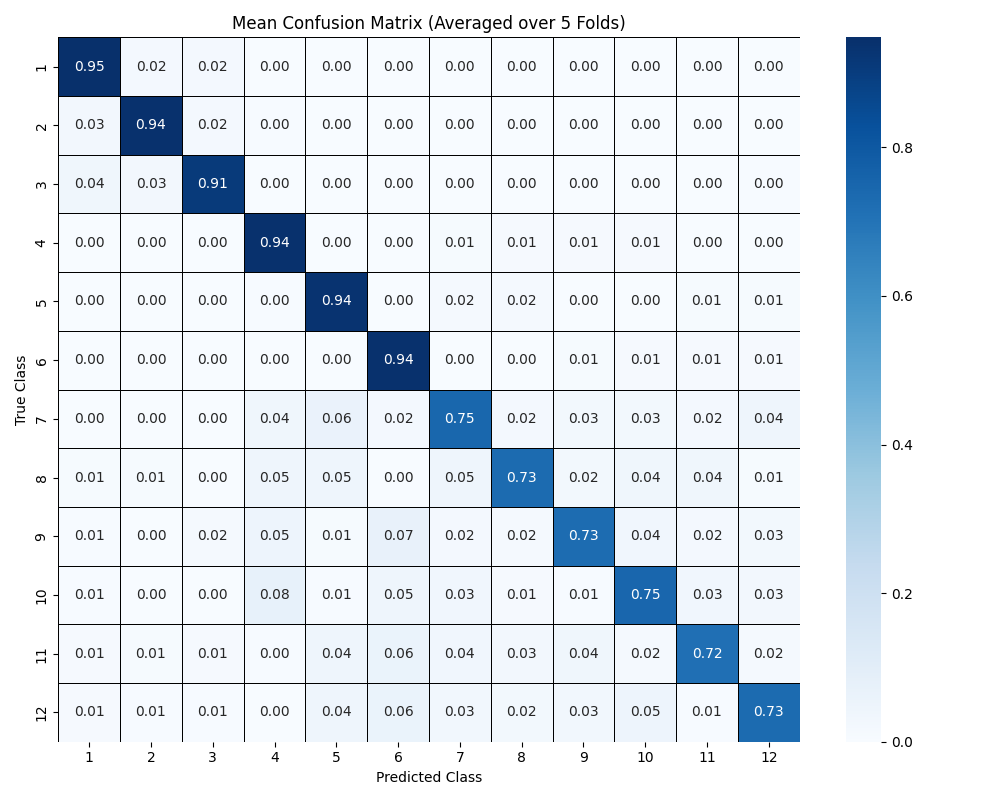
\includegraphics[width=1\textwidth]{Images/Chapter4/confusion-main.png}
  \caption{ماتریس درهم‌ریختگی میانگین برای حالت ۸۰ درصد داده آموزشی}
  \label{fig:confusion-main}
\end{figure}

همانطور که در شکل \ref{fig:confusion-main} دیده می‌شود، فعالیت‌های ۱ تا ۶ دارای دقت‌های بسیار بالا هستند که نشان دهنده‌ی عملکرد بسیار خوب مدل در مواجهه با این داده‌ها می‌باشد. اما فعالیت‌های ۷ تا ۱۲ که بیانگر تغییرات در فعالیت هستند دقت‌های پایین‌تری دارند. چرا که در بازه زمانی کوتاه رخ می‌دهند و وضعیت بدن را از حالتی به حالت دیگر تغییر می‌دهند، که تشخیص دقیق مرزهای آن‌ها برای مدل دشوارتر است.

بین کلاس‌های ۱، ۲ و ۳ درهم‌ریختگی متقابل کوچک در حدود \%۴ وجود دارد.
به عنوان مثال، راه رفتن با احتمال \%۳ به عنوان بالا رفتن از پله و \%۴ به عنوان پایین آمدن از پله اشتباه گرفته شده است. این اشتباهات منطقی هستند زیرا این فعالیت‌ها از لحاظ نوع حرکت (راه رفتن) مشابهند. کلاس‌های ۴ و ۵ و ۶ هم عمدتا با یکدیگر اشتباه گرفته نمی‌شوند که این امر نشان می‌دهد مدل در تمایز بین این حالات بدن، بسیار قدرتمند عمل می‌کند.

اما بیشترین اشتباهات در پیش‌بینی کلاس‌های ۷ تا ۱۲ دیده می‌شود:
\begin{enumerate}
    \item \textbf{پیش‌بینی ۴ به جای ۷:} ایستادن به نشستن شامل لحظاتی است که فرد در نهایت نشسته است. مدل در تشخیص لحظه انتقال ضعیف عمل کرده و صرفاً وضعیت نهایی (نشستن) را پیش‌بینی کرده است.
    \item \textbf{پیش‌بینی ۸ به جای ۷:} اشتباه گرفتن دو فرآیند معکوس (انتقال از ایستادن به نشستن با انتقال از نشستن به ایستادن). این به دلیل شباهت‌های حرکتی در میانه انتقال است.
    \item \textbf{پیش‌بینی ۵ به جای ۸:} مشابه مورد بالا، مدل به جای انتقال، وضعیت نهایی (ایستادن) را پیش‌بینی کرده است.
    \item \textbf{پیش‌بینی ۷ به جای ۸:} اشتباه گرفتن دو فرآیند معکوس.
    \item \textbf{پیش‌بینی ۹ و ۱۰ به جای ۱۱:} فرد قبل از خوابیدن از حالت ایستاده معمولاً می‌نشیند. مدل در تشخیص زنجیره حرکتی ضعیف عمل کرده و بخش‌های میانی انتقال (مثل نشستن) را به اشتباه پیش‌بینی کرده است (\%۴ به نشستن و \%۶ به خوابیدن).
    \item \textbf{پیش‌بینی ۱۱ به جای ۱۲:} اشتباه گرفتن دو فرآیند معکوس.
\end{enumerate}

در مجموع، نتایج این بخش به وضوح نشان می‌دهد که روش پیشنهادی نه تنها بر محدودیت‌های یادگیری کاملا نظارت‌شده در شرایط کمبود داده فائق می‌آید، بلکه در مقایسه مستقیم با روش پایه‌ی اخیر نیز در اکثر موارد عملکردی بهتر ارائه می‌دهد. این نتایج، پتانسیل بالای مدل را در سناریوی درون-مجموعه‌ای تأیید می‌کند. در بخش بعد، این ارزیابی را یک گام فراتر برده و عملکرد مدل را در سناریوی چالش‌برانگیزتر یادگیری انتقالی خواهیم سنجید.

\subsection{نتایج آزمایش‌های بین‌مجموعه‌ای}

در این بخش، به بررسی نتایج حاصل از سناریوی دوم، یعنی پیش‌آموزش خودنظارتی بر روی مجموعه داده \lr{MobiAct} و تنظیم دقیق مدل بر روی مجموعه داده‌ی \lr{HAPT}
می‌پردازیم. نتایج دقیق این آزمایش‌ها در جدول
\ref{tab:inter-dataset-comparison}
ارائه شده است. این جدول، میانگین و انحراف معیار امتیاز
\lr{F1}
و امتیاز کاپا را به ازای استفاده از ۲۰، ۴۰، ۶۰ و ۸۰ درصد از داده‌های آموزشی برچسب‌دار، پس از ۵ بار تکرار آزمایش، نمایش می‌دهد

\begin{table}[ht]
\centering
\caption{نتایج عملکرد مدل در سناریوی بین‌مجموعه‌ای بر اساس درصدهای مختلف داده آموزشی}
\label{tab:inter-dataset-comparison}
\begin{tabular}{clll}
    \toprule
    \textbf{درصد داده} & \textbf{روش} & \textbf{امتیاز \lr{F1}} & \textbf{امتیاز کاپا} \\
    \midrule
    \multirow{3}{*}{\%۲۰} 
    & کاملا نظارت‌شده & $0.439 \pm 0.006$ & $0.316 \pm 0.007$ \\
    & روش پایه \cite{taghanaki2023self} & $0.591 \pm 0.006$ & $0.489 \pm 0.007$ \\
    & روش پیشنهادی & $\boldsymbol{0.602 \pm 0.006}$ & $\boldsymbol{0.560 \pm 0.008}$ \\
    \midrule
    \multirow{3}{*}{\%۴۰} 
    & کاملا نظارت‌شده & $0.619 \pm 0.008$ & $0.521 \pm 0.008$ \\
    & روش پایه \cite{taghanaki2023self} & $0.743 \pm 0.010$ & $0.676 \pm 0.011$ \\
    & روش پیشنهادی & $\boldsymbol{0.763 \pm 0.011}$ & $\boldsymbol{0.701 \pm 0.015}$ \\
    \midrule
    \multirow{3}{*}{\%۶۰} 
    & کاملا نظارت‌شده & $0.770 \pm 0.008$ & $0.710 \pm 0.010$ \\
    & روش پایه \cite{taghanaki2023self} & $0.831 \pm 0.007$ & $0.789 \pm 0.009$ \\
    & روش پیشنهادی & $\boldsymbol{0.863 \pm 0.007}$ & $\boldsymbol{0.830 \pm 0.009}$ \\
    \midrule
    \multirow{3}{*}{\%۸۰} 
    & کاملا نظارت‌شده & $0.893 \pm 0.007$ & $0.869 \pm 0.008$ \\
    & روش پایه \cite{taghanaki2023self} & $0.887 \pm 0.007$ & $0.863 \pm 0.008$ \\
    & روش پیشنهادی & $\boldsymbol{0.902 \pm 0.004}$ & $\boldsymbol{0.886 \pm 0.006}$ \\
    \bottomrule
\end{tabular}
\end{table}

\begin{figure}[ht!]
    \centering
    \begin{subfigure}[b]{0.49\textwidth}
        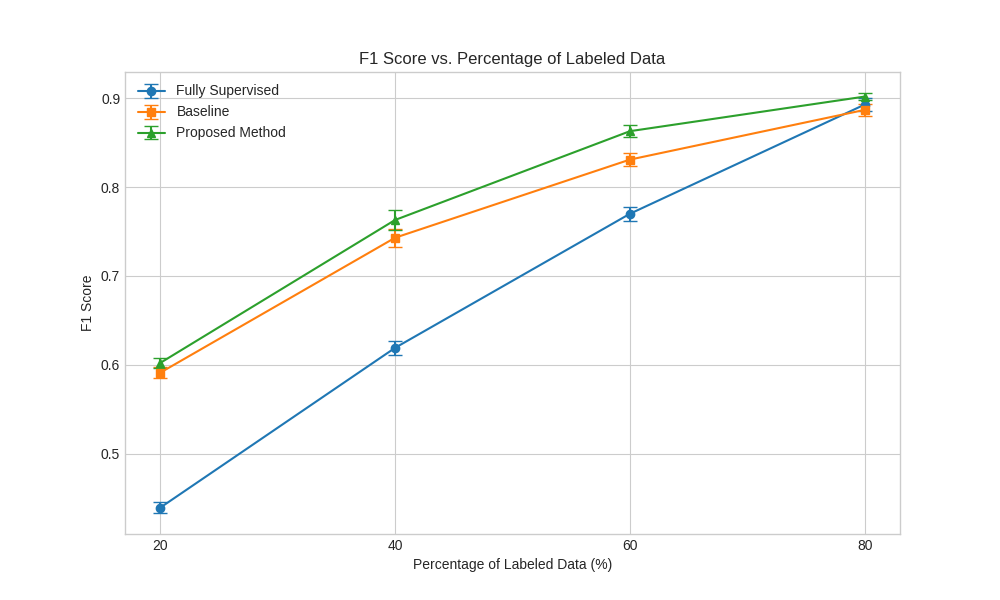
\includegraphics[width=\textwidth]{Images/Chapter4/transfer-results-f1.png}
    \end{subfigure}
    \hfill % ایجاد فاصله بین دو عکس
    \begin{subfigure}[b]{0.49\textwidth}
        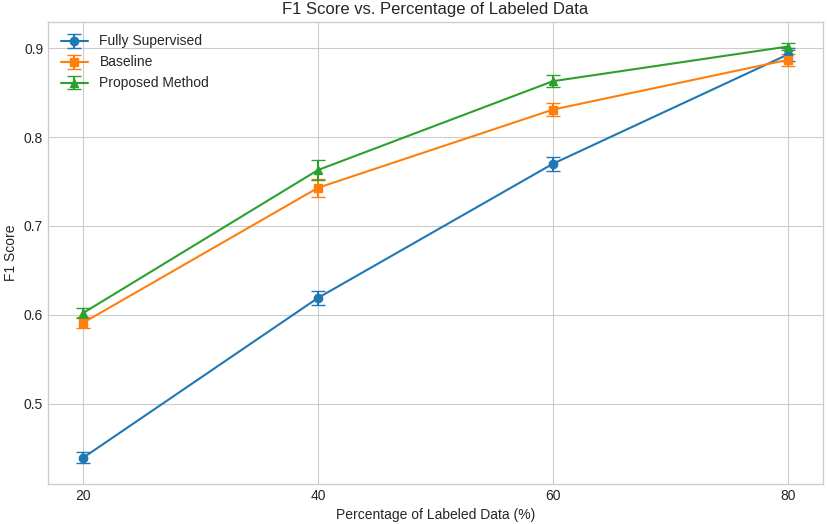
\includegraphics[width=\textwidth]{Images/Chapter4/transfer-results-kappa.png}
    \end{subfigure}
    \caption{مقایسه امتیاز \lr{F1} (راست) و امتیاز کاپا (چپ) برای روش‌های مختلف بر اساس درصدهای متفاوت داده‌های آموزشی.}
    \label{fig:transfer-results}
\end{figure}

تحلیل نتایج ارائه شده در جدول \ref{tab:inter-dataset-comparison}، به ویژه هنگامی که در کنار نتایج آزمایش‌های درون-مجموعه‌ای (جدول \ref{tab:intra-dataset-comparison}) قرار می‌گیرد، یافته‌های بسیار مهمی را در مورد قدرت تعمیم و پایداری مدل‌ها آشکار می‌سازد.

اولین مشاهده در تحلیل این جدول، برتری کامل و مداوم روش پیشنهادی بر هر دو روش دیگر در تمامی سطوح داده‌ی برچسب‌دار است. برخلاف سناریوی قبلی که در سطح \%۴۰ داده، رقابت بسیار نزدیک بود، در این سناریوی بین-مجموعه‌ای، مدل پیشنهادی در تمام آزمون‌ها با اختلاف معناداری بهترین عملکرد را به ثبت رسانده است. این موضوع نشان می‌دهد که بازنمایی‌های آموخته‌شده توسط روش پیشنهادی از مجموعه داده \lr{MobiAct}، برای انتقال به دامنه جدید (مجموعه داده \lr{HAPT}) کارآمدتر و قابل‌استفاده‌تر بوده‌اند.

نکته کلیدی و بسیار قابل تأمل، مقایسه مستقیم عملکرد مدل‌ها بین دو سناریو است. مشاهده می‌شود که امتیازات \lr{F1} و کاپا برای هر دو روش خودنظارتی در سناریوی بین‌مجموعه‌ای به طور کلی کمتر از سناریوی درون‌مجموعه‌ای است. مجموعه داده‌های \lr{MobiAct} و \lr{HAPT} اگرچه هر دو به شناسایی فعالیت انسان می‌پردازند، اما در جزئیاتی نظیر
نوع و محل قرارگیری سنسورها، مجموعه فعالیت‌های ثبت‌شده و مشخصات شرکت‌کنندگان تفاوت‌هایی دارند. این تفاوت‌ها باعث ایجاد اختلاف در توزیع آماری داده‌ها شده و باعث می‌شود بازنمایی‌های آموخته‌شده از یک دامنه، به طور کامل به دامنه‌ی دیگر قابل انتقال نباشند.

با این حال، با وجود اینکه هر دو روش خودنظارتی تحت تاثیر تغییر دامنه دچار افت عملکرد شدند، اما میزان این افت برای روش پایه به مراتب شدیدتر بوده است. این یافته نشان می‌دهد که روش پیشنهادی مقاومت بیشتری در برابر تغییر دامنه دارد و قادر به یادگیری بازنمایی‌های عمومی‌تر و مستقل از دامنه است. در حالی که روش پایه ممکن است ویژگی‌هایی را آموخته باشد که بیش از حد به خصوصیات مجموعه داده \lr{MobiAct} وابسته بوده‌اند، روش پیشنهادی توانسته است الگوهای کلی‌تری را استخراج کند که حتی پس از انتقال به یک دامنه جدید نیز کارایی بالاتری از خود نشان می‌دهند.

\begin{figure}[htb!]
  \centering
  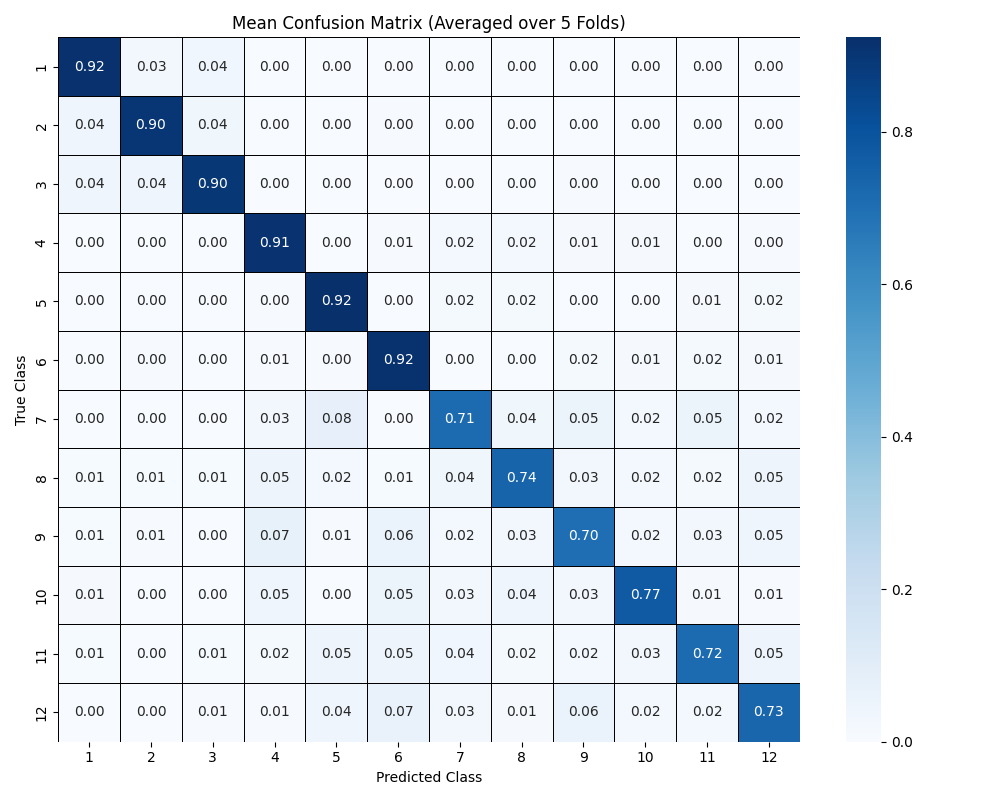
\includegraphics[width=1\textwidth]{Images/Chapter4/confusion-transfer.png}
  \caption{ماتریس درهم‌ریختگی میانگین برای حالت ۸۰ درصد داده آموزشی در یادگیری انتقالی}
  \label{fig:confusion-transfer}
\end{figure}

تحلیل‌های مربوط به ماتریس درهم‌ریختگی شکل \ref{fig:confusion-transfer} عینا مانند ماتریس درهم‌ریختگی شکل \ref{fig:confusion-main} می‌باشند و مدل به همان نسبت و با دقت کمتر همان نقاط قوت و نقاط ضعف را از خود نشان داده است.

در نهایت، نتایج این بخش نشان می‌دهد که اگرچه فرضیه ساده "پیش‌آموزش روی داده بیشتر همیشه بهتر است" به دلیل وجود شکاف دامنه به چالش کشیده می‌شود، اما همین چالش، نقطه قوت اصلی روش پیشنهادی را آشکار می‌سازد: پایداری\LTRfootnote{Robustness} و قابلیت تعمیم بالاتر در شرایط واقعی که داده‌های آموزش و آزمون ممکن است از توزیع‌های متفاوتی آمده باشند. این ویژگی، ارزش عملیاتی مدل پیشنهادی را به شدت افزایش می‌دهد.

\section{جزئیات اجرا}

برای آموزش مدل‌ها از یک کارت گرافیک \lr{NVIDIA Tesla P100} استفاده شده است. جزئیات زمان اجرای پیش‌آموزش مدل‌ها به شرح زیر می‌باشد:
\begin{itemize}
    \item \textbf{مجموعه داده \lr{HAPT}:} هر دوره از پیش‌آموزش کدگذار سیگنال حدود ۱۲۵ ثانیه و هر دوره از پیش‌آموزش کدگذار اسکالوگرام حدود ۲۶۰ ثانیه به‌طول انجامید. نتیجتا پیش‌آموزش کامل کدگذار سیگنال حدود ۳ و نیم ساعت و کدگذار اسکالوگرام حدود ۵ و نیم ساعت به‌طول انجامید.
    \item \textbf{مجموعه داده \lr{MobiAct}:} هر دوره از پیش‌آموزش کدگذار سیگنال حدود ۱۳۰۰ ثانیه و هر دوره از پیش‌آموزش کدگذار اسکالوگرام حدود ۲۸۰۰ ثانیه به‌طول انجامید. نتیجتا پیش‌آموزش کامل کدگذار سیگنال حدود ۳۶ ساعت و کدگذار اسکالوگرام حدود ۵۸ ساعت به‌طول انجامید.
\end{itemize}

یکی از معیارهای کلیدی برای نظارت بر فرایند پیش‌آموزش و اطمینان از یادگیری بازنمایی‌های مفید، رصد کردن مقدار تابع هزینه روش \lr{SwAV} بود. اگر مقدار این تابع هزینه به عدد ثابت
$\log(K)$ (که در آن $K$ تعداد خوشه‌ها است) نزدیک شود، این امر نشان‌دهنده‌ی عدم یادگیری بازنمایی‌های معنادار توسط مدل است. دلیل این پدیده به شرح زیر است:

تابع هزینه \lr{SwAV}، همانطور که در معادله \ref{eq:swav-cross-entropy} نشان داده شد، بر اساس آنتروپی متقاطع عمل می‌کند. در این میان، بردار احتمال $p$ از خروجی یک تابع سافت‌مکس بر روی امتیازات شباهت بین بازنمایی شبکه ($z$) و مراکز خوشه‌ها به دست می‌آید (معادله \ref{eq:swav-p-calculation}). در صورتی که مدل در حال یادگیری نباشد (مثلاً به دلیل تنظیم نامناسب ابرپارامترها)، بازنمایی خروجی آن حاوی اطلاعات مفیدی نخواهد بود. در نتیجه، امتیاز شباهت این بازنمایی با تمام $K$
مرکز خوشه تقریبا یکسان خواهد بود. هنگامی که ورودی‌های یک تابع سافت‌مکس مقادیر یکسانی داشته باشند، خروجی آن یک توزیع احتمال یکنواخت خواهد بود، یعنی $p_k \approx \frac{1}{K}$ برای تمام خوشه‌ها. با جایگزین کردن $p_k$ در فرمول هزینه داریم:
\begin{equation}
    L = - \sum_{k=1}^{K} q_k \log \left( \frac{1}{K} \right) = \log(K) \sum_{k=1}^{K} q_k
\end{equation}
و از آنجا که $q$ نیز خود یک توزیع احتمال است، جمع تمام $q_k$ برابر با ۱ می‌شود و مقدار نهایی هزینه به فرم $L = \log(K)$ در می‌آید. بنابراین، وقتی مدل یادگیری را به درستی انجام نمی‌دهد، هزینه به پایین‌ترین حد ممکن برای یک حدس تصادفی، یعنی 
$\log(K)$ می‌رسد.

بنابراین، مقدار $\log(K)$ به عنوان خط پایه برای یک مدل تصادفی\LTRfootnote{Random Baseline} عمل می‌کند. در یک آموزش موفق، انتظار می‌رود که مقدار هزینه به سرعت از این عدد فاصله گرفته و به سمت مقادیر کمتر کاهش یابد. نزدیک شدن یا باقی ماندن هزینه در این سطح، هشداری مبنی بر عدم یادگیری مدل است.

\section{جمع‌بندی}

در این فصل، عملکرد مدل پیشنهادی از طریق مجموعه‌ای از آزمایش‌های جامع مورد ارزیابی قرار گرفت. ابتدا، مجموعه داده‌های مورد استفاده به عنوان بستر آزمایش‌ها معرفی شدند و سپس جزئیات پیاده‌سازی، شامل مراحل پیش‌پردازش داده‌ها، فرایند آموزش دومرحله‌ای، ابرپارامترها و معیارهای ارزیابی تشریح گردید. نتایج در دو سناریوی اصلی ارائه شد: درون‌مجموعه‌ای و بین‌مجموعه‌ای. در سناریوی درون‌مجموعه‌ای، برتری آشکار رویکرد خودنظارتی پیشنهادی نسبت به یادگیری کاملا نظارت‌شده، به‌ویژه در شرایط کمبود داده، به اثبات رسید و در اکثر موارد عملکرد بهتری نسبت به روش پایه داشت. مهم‌تر از آن، در سناریوی چالش‌برانگیز بین‌مجموعه‌ای (یادگیری انتقالی)، مدل پیشنهادی پایداری و قابلیت تعمیم بالاتری از خود به نمایش گذاشت و با اختلاف معناداری نسبت به روش پایه، برتری خود را در تمام سطوح داده‌های برچسب‌دار تثبیت کرد. این یافته‌ها نشان می‌دهد که مدل پیشنهادی قادر به یادگیری بازنمایی‌های غنی، عمومی و مقاوم در برابر تغییر دامنه است.
